\documentclass[a4paper,12pt,BCOR2cm,DIV12]{scrartcl}
\usepackage{graphics}
\usepackage{verbatim}
\usepackage{setspace}
\usepackage{fancyhdr}
\pagestyle{fancy}
\lhead{}
\chead{}
\rhead{}
\lfoot{}
\cfoot{--\thepage--}
\rfoot{}
\renewcommand{\headrulewidth}{0.0pt}
\renewcommand{\footrulewidth}{0.0pt}

\makeatletter
\renewenvironment{thebibliography}[1]
      {%
       \@mkboth{\MakeUppercase\refname}{\MakeUppercase\refname}%
       \list{\@biblabel{\@arabic\c@enumiv}}%
            {\settowidth\labelwidth{\@biblabel{#1}}%
             \leftmargin\labelwidth
             \advance\leftmargin\labelsep
             \@openbib@code
             \usecounter{enumiv}%
             \let\p@enumiv\@empty
             \renewcommand\theenumiv{\@arabic\c@enumiv}}%
       \sloppy
       \clubpenalty4000
       \@clubpenalty \clubpenalty
       \widowpenalty4000%
       \sfcode`\.\@m}
      {\def\@noitemerr
        {\@latex@warning{Empty `thebibliography' environment}}%
       \endlist}
\makeatother

\author{Felix Wiemann}
\title{Simulation of Page Replacement Algorithms}


\begin{document}

\newpage

\begin{center}
{
  \thispagestyle{empty}

  \vspace*{3cm}
  
  \Huge
  Simulation of Page\\
  Replacement Algorithms

  \vspace{3cm}

  \Large
  Felix Wiemann

}
\end{center}

\newpage

\thispagestyle{empty}

\tableofcontents

\newpage

\section{Abstract}

This is a facharbeit about the simulation of page replacement
algorithms.  This means that it focuses mainly on the
\emph{simulation}, not on the page replacement algorithms themselves.
Basic knowledge of memory management systems is presumed.

For a good introduction to the topic, I recommend reading
\cite{Tan01}, which comprises a chapter about memory management.

\section{Page replacement algorithms}

This section gives a very short overview of the page replacement
algorithms which can be simulated with the scripts and their
implementation on real hardware.

\subsection{Optimal}

The optimal algorithm replaces the page which will not be accessed for
the longest time.

To do this, it needs to look into the future, thus it is
unimplementable in reality.  However, it is quite useful for
comparison purposes in simulations, because in a simulated
environment, it is possible to predefine the order in which pages are
accessed.  Using the optimal algorithm, you can see how ``real''
algorithms perform compared to the optimum.

\subsection{Least Recently Used (LRU)}

The ``least recently used'' (LRU) algorithm replaces the page which
has not been accessed for the longest time.

It performs very well, but it is difficult to implement.  There are
several implementations of it:

\begin{enumerate}

\item Every time a page is read, it is moved to the head of the list.
  The next page to replace is the one at the tail of the list.  It is
  very hard to perform this task so fast that it does not slow down
  the whole system, because memory accesses occur very frequently.

\item We use a bit matrix consisting of $n*n$ bits, where $n$ is the
  number of physical pages in memory---refer to \cite{Tan01} for
  details on this implementation.  If there are many pages, the bit
  matrix grows very big.

\item Every time a page is read, the current time is stored in a
  variable of this page.  The next page to swap out is the one with
  the lowest time of last access.  This is hardly implementable
  because the timer needs more than 32 bit to be fine-granular enough
  and finding the page with the lowest access time is very expensive.

\end{enumerate}

\subsection{First In First Out (FIFO)}

The FIFO (first-in-first-out) algorithm is extremely simple: It
removes the page with the earliest creation time.

This can be implemented using a list: New pages are inserted at the
head of the list, and the page at the tail is swapped out.

Another implementation is using a ring (usually referred to as
``clock''): Every time a page has to be replaced, the page the pointer
points at is swapped out and at the same place the new page is swapped
in.  After this, the pointer moves to the next page.

The FIFO algorithm's performance is rather bad.

\subsection{Second Chance}

The second-chance algorithm is very similar to FIFO.  However, it
interferes with the accessing process: Every page has, in addition to
its ``dirty bit'', a ``referenced bit'' (r-bit).  Every time a page is
accessed, the r-bit is set.

The replacement process works like FIFO, except that when a page's
r-bit is set, instead of replacing it, the r-bit is unset, the page is
moved to the list's tail (or the pointer moves to the next page,
resp.) and the next page is examined.

Second Chances performs better than FIFO, but it is still far from
optimal.

\subsection{Aging}

The aging algorithm is somewhat tricky: It uses a bit field of $w$
bits for each page in order to track its accessing profile.

Every time a page is read, the \emph{first} (i.e.\ most significant)
bit of the page's bit field is set.  Every $n$ instructions all pages'
bit fields are right-shifted by one bit.

The next page to replace is the one with the lowest (numerical) value
of its bit field.  If there are several pages having the same value,
an arbitrary page is chosen.

The aging algorithm works very well in many cases, and sometimes even
better than LRU, because it looks behind the last access.  It
furthermore is rather easy to implement, because there are no
expensive actions to perform when reading a page.  However, finding
the page with the lowest bit field value usually takes some time.
Thus, it might be necessary to predetermine the next page to be
swapped out in background.

\subsection{Not Recently Used (NRU)}

The NRU (not-recently-used) algorithm uses an r-bit for every page.
Every time a page is read, the r-bit is set.  Periodically, all r-bits
are unset.  When a page fault occurs, an arbitrary page with r-bit
unset is swapped out.

NRU is actually Aging with a bit field width of 1, and it does not
perform very well.

\section{Simulation of page replacement algorithms}

Now we start with the really interesting part: The \emph{simulation}
of page replacement algorithms.

\subsection{How to simulate}

The scripts to simulate the page replacement algorithms are written in
Python.  They have been tested with Python-2.2.3, but other versions
might work as well.

There are four modules, {\tt mms}, {\tt algorithms}, {\tt access} and
{\tt simulate}, and {\tt demo}, a demonstration script.

After reading this section I recommend executing {\tt demo.py} in
order to get an idea of how it works in practice.

\subsubsection{MMS}

The module {\tt mms} contains a generic (abstract) class {\tt MMS},
which represents a memory management system.  All page replacement
algorithms are classes derived from {\tt MMS}.

{\tt MMS}' constructor takes one parameter, the number of physical
pages.  (The number of virtual pages is unlimited.)

The method {\tt read} reads a page.  It takes one parameter, the
virtual page number.  If the page is already contained in memory, it
does nothing.  (Of course, this behavior may be changed by derived
classes.)  If the page is not contained in memory, the method {\tt
pagefault} is called.

If the memory is full, {\tt pagefault} calls {\tt swapout}, which is
not defined in {\tt MMS} and has to be implemented by derived classes.
After this, {\tt pagefault} calls {\tt create}, which creates a new page in
memory.  Derived classes might implement additional behavior for
{\tt create}.

The method {\tt output} is simply used for outputting the virtual page
numbers in a human-readable format.  By default, it outputs the next
page to swap out last, however this behavior might be undesirable for
some non-stack algorithms like Second Chance, which should overwrite
{\tt output} for better convenience.

Every time a page is swapped in (or out), {\tt pagefault} increments
{\tt swapin} (or {\tt swapout}, resp.), so that you can measure the
algorithms' performances.

\subsubsection{Algorithms}

The module {\tt algorithms} contains from {\tt mms.MMS} derived
classes which implement various page replacement algorithms.

The classes {\tt FIFO}, {\tt SecondChance} and {\tt
LRU} are self-explanatory.

{\tt Optimal} needs to get a list of virtual page numbers which will
we accessed, either as second parameter of the constructor or as
assignment to the {\tt alist} attribute.  The algorithm will only be
optimal if the order of read pages is the same as in {\tt alist}.

{\tt Aging} may get the bit field width and shifting frequency as
second and third constructor-parameter or as parameters to the method
{\tt configure}.  (``Shifting frequency'' means the number of
read-instructions between the shifts.)  Defaults for both are
provided.

{\tt NRU} is derived from {\tt Aging} and uses a bit field length of
1, regardless of its configuration.

\subsubsection{Access}

The module {\tt access} provides helper functions to simulate memory
accessing behavior of real programs.

Some general notes for all functions in this module: {\tt mem} is a
list of virtual page numbers representing the whole allocated memory.
{\tt ws} is a list of virtual page numbers representing a program's
working set and may be contained in {\tt mem}.  {\tt probab} is a
probability in the range of 0 to 1.  {\tt rand} is a random number
generator, e.g.\ the module {\tt random} or an instance of {\tt
random.Random}.

The function {\tt access(mem, ws, rand, probab)} returns a page.  With
a probability of {\tt probab}, the returned page is contained in {\tt
ws}.  Otherwise, it is contained in {\tt mem} but not in {\tt ws}.

{\tt makealist(mem, ws, rand, probab, length)} returns a list of {\tt
length} pages to access.  Basically, it works like {\tt access},
except that \emph{exactly} {\tt round((1 - probab) * length)} pages
are contained in {\tt mem} but not in {\tt ws} and all other pages are
contained in {\tt ws}, so that random inaccuracies are avoided.

{\tt wsmake(mem, rand, size)} returns a working set of {\tt size}
pages which are all contained in {\tt mem}.

{\tt wsmove(mem, ws, rand)} removes one page from {\tt ws} and adds a
different, randomly chosen page from {\tt mem} to {\tt ws}.

{\tt wsextend(mem, ws, rand)} adds a random page from {\tt mem} to
{\tt ws}.

{\tt wsshrink(ws, rand)} removes a random page from {\tt ws}.

None of the four {\tt ws}-functions touch {\tt mem}, and, when adding
a page to {\tt ws}, they ensure that no page is contained more than
once in {\tt ws}.

\subsubsection{Simulate}

The module {\tt simulate} has only one function, {\tt simulate(mms,
alist, skip=0)}, which invokes {\tt mms.read} for all pages in {\tt
alist}.  It returns the ratio of page faults to accesses, leaving the
first {\tt skip} accesses out of consideration.  {\tt skip} defaults
to 0.

\subsection{What to simulate}

This section deals with what exactly to simulate.

\subsubsection{Hardware}

If the hardware is still being designed, an important point is how to
support the algorithm.

E.g., without the ability to perform any action after reading a page,
there is not much more left than FIFO.

If the hardware is able to reorder elements of a list at every
read-instruction, it is possible to implement LRU.

If there are not many pages, it might be a good idea to choose the
bit-matrix implementation of LRU or to supply automatically shifting
bit-fields for every page in order to support Aging.

\subsubsection{Software}

Now we can start creating profiles of the programs which will run on
the system.  E.g., we could generate access lists by tracking a (real)
program's memory access behavior.

Or we could analyse the source of the programs in order to answer
questions like these: Does the program have a working set at all?  (If
it does not, we simply do not need to care of a decent page
replacement algorithm.)  If it does, how does the working set change
over time?  Does it have a constant size?  Does it move?  And so on.
Based on these parameters, we can create access lists which
approximate the program's memory accessing behavior using the {\tt
access} module.

\subsubsection{Algorithms}

Based on the previously defined hardware environment, we select
algorithms which can run in that environment, or we even implement
some more complex algorithms specific to our hardware.

Then we simulate the algorithms using the {\tt simulate} module.

\subsubsection{Example 1}

The hardware has 64 pages of memory and shall be suitable for
applications with a working set size of up to 60 pages.  The
applications will use the working set at about 95\% of their accesses.

First, let us presume that our hardware has unlimited abilities, so
that we can compare all algorithms in order to see if there is a cheap
possibility to implement a good page replacement algorithm.

We create a diagram.  Read the source of {\tt makediagram1.py} on how
to exactly do this.

\vspace{5mm}

%GNUPLOT: LaTeX picture with Postscript
\begin{picture}(0,0)%
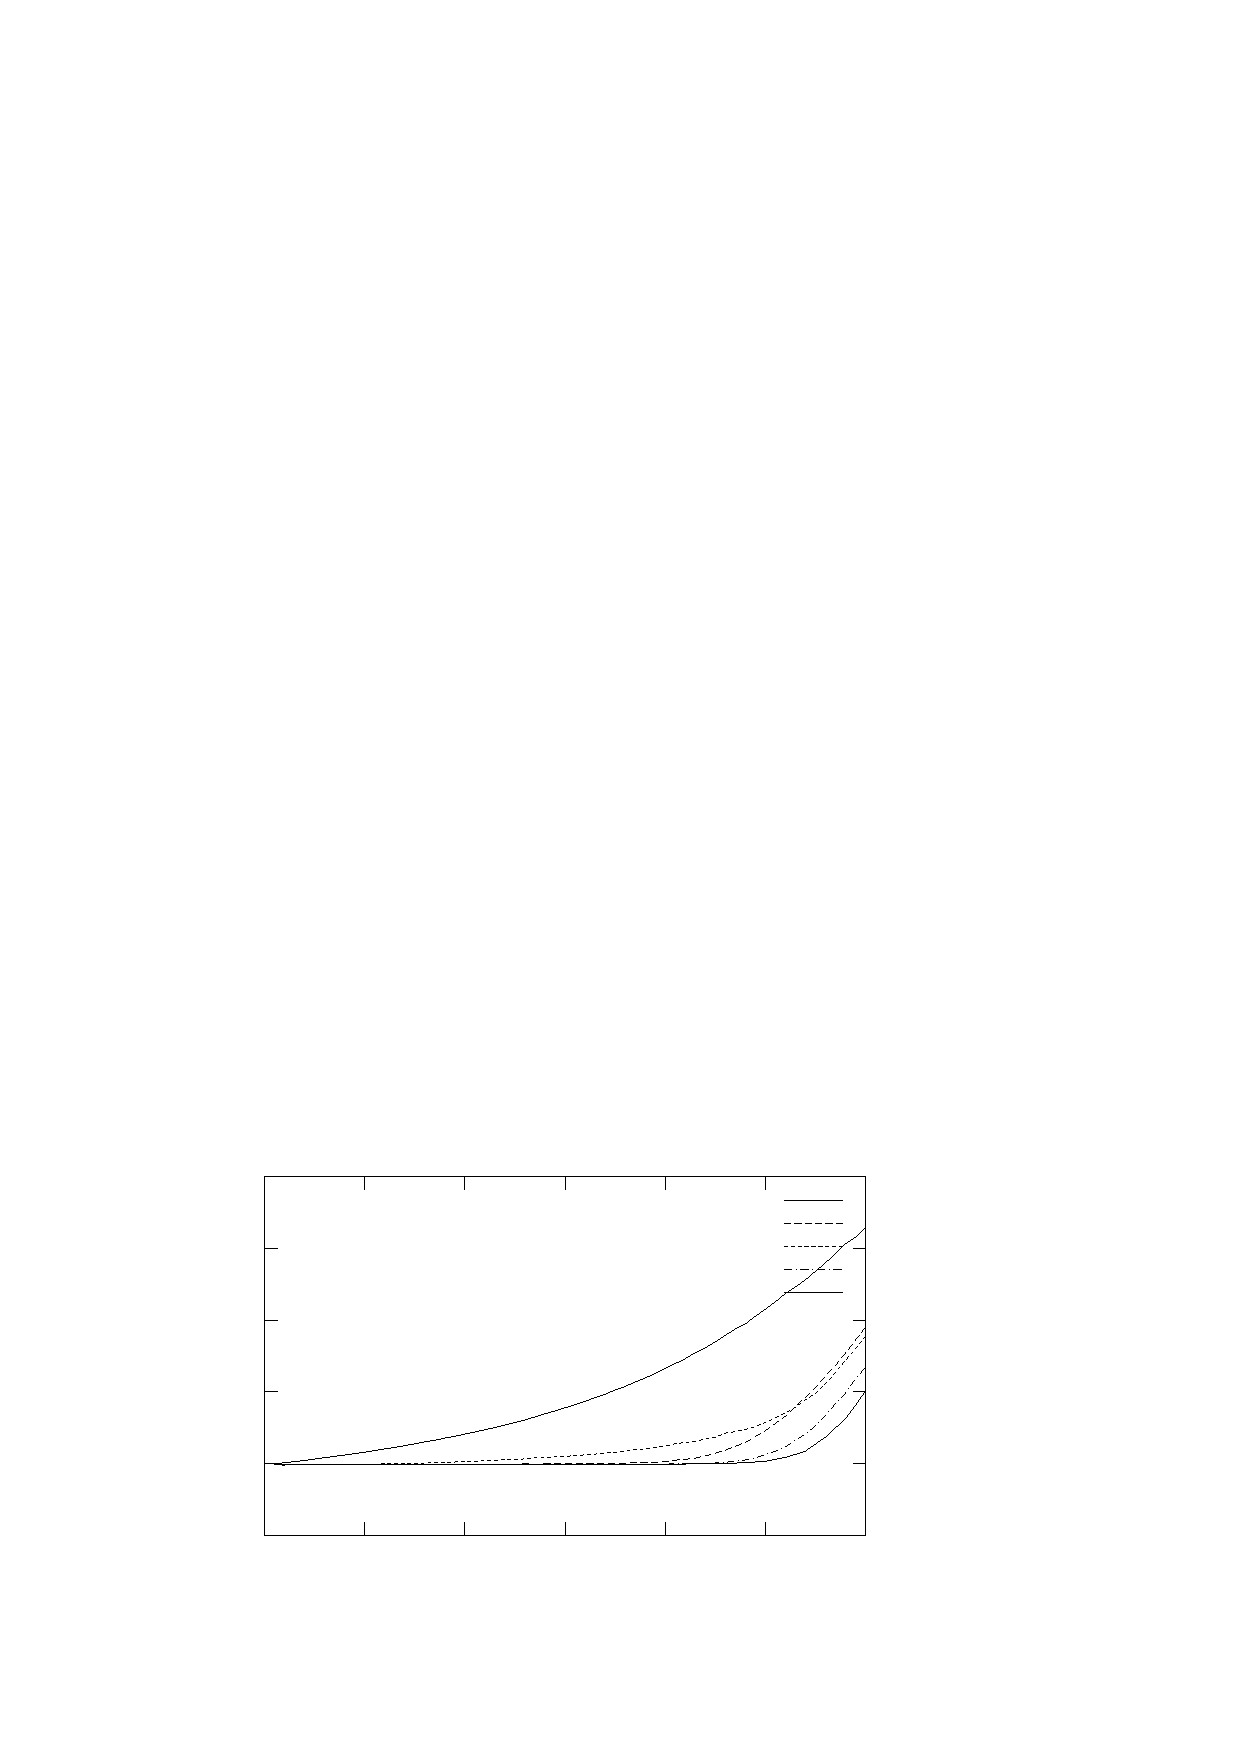
\includegraphics{diagram1}%
\end{picture}%
\setlength{\unitlength}{0.0200bp}%
\begin{picture}(18000,10800)(0,0)%
\put(2475,1650){\makebox(0,0)[r]{\strut{} 0}}%
\put(2475,3370){\makebox(0,0)[r]{\strut{} 0.05}}%
\put(2475,5090){\makebox(0,0)[r]{\strut{} 0.1}}%
\put(2475,6810){\makebox(0,0)[r]{\strut{} 0.15}}%
\put(2475,8530){\makebox(0,0)[r]{\strut{} 0.2}}%
\put(2475,10250){\makebox(0,0)[r]{\strut{} 0.25}}%
\put(2750,1100){\makebox(0,0){\strut{} 0}}%
\put(5154,1100){\makebox(0,0){\strut{} 10}}%
\put(7558,1100){\makebox(0,0){\strut{} 20}}%
\put(9962,1100){\makebox(0,0){\strut{} 30}}%
\put(12367,1100){\makebox(0,0){\strut{} 40}}%
\put(14771,1100){\makebox(0,0){\strut{} 50}}%
\put(17175,1100){\makebox(0,0){\strut{} 60}}%
\put(550,5950){\rotatebox{90}{\makebox(0,0){\strut{}ratio of page faults to accesses}}}%
\put(9962,275){\makebox(0,0){\strut{}working set size in pages}}%
\put(14950,9675){\makebox(0,0)[r]{\strut{}FIFO}}%
\put(14950,9125){\makebox(0,0)[r]{\strut{}SecondChance}}%
\put(14950,8575){\makebox(0,0)[r]{\strut{}NRU}}%
\put(14950,8025){\makebox(0,0)[r]{\strut{}LRU}}%
\put(14950,7475){\makebox(0,0)[r]{\strut{}Aging}}%
\end{picture}%
\endinput


\vspace{5mm}

FIFO performs really bad, Second Chance and NRU (both using only the
r-bit) perform better and the complex algorithms LRU and Aging are
by far the best ones.

\subsubsection{Example 2}

Another example:

Aging is a very good algorithm and could be supported by a hardware we
are currently designing.  Our hardware has a memory size of 6 pages,
and the bit fields utilized by the Aging algorithm consist of 4 bits.

The applications which will run on our system will have a working set
size of 5 pages and a very large allocated virtual memory.

Now we want to know which shifting frequency is best for this
environment.  We create a diagram using {\tt makediagram2.py}.

\vspace{5mm}

%GNUPLOT: LaTeX picture with Postscript
\begin{picture}(0,0)%
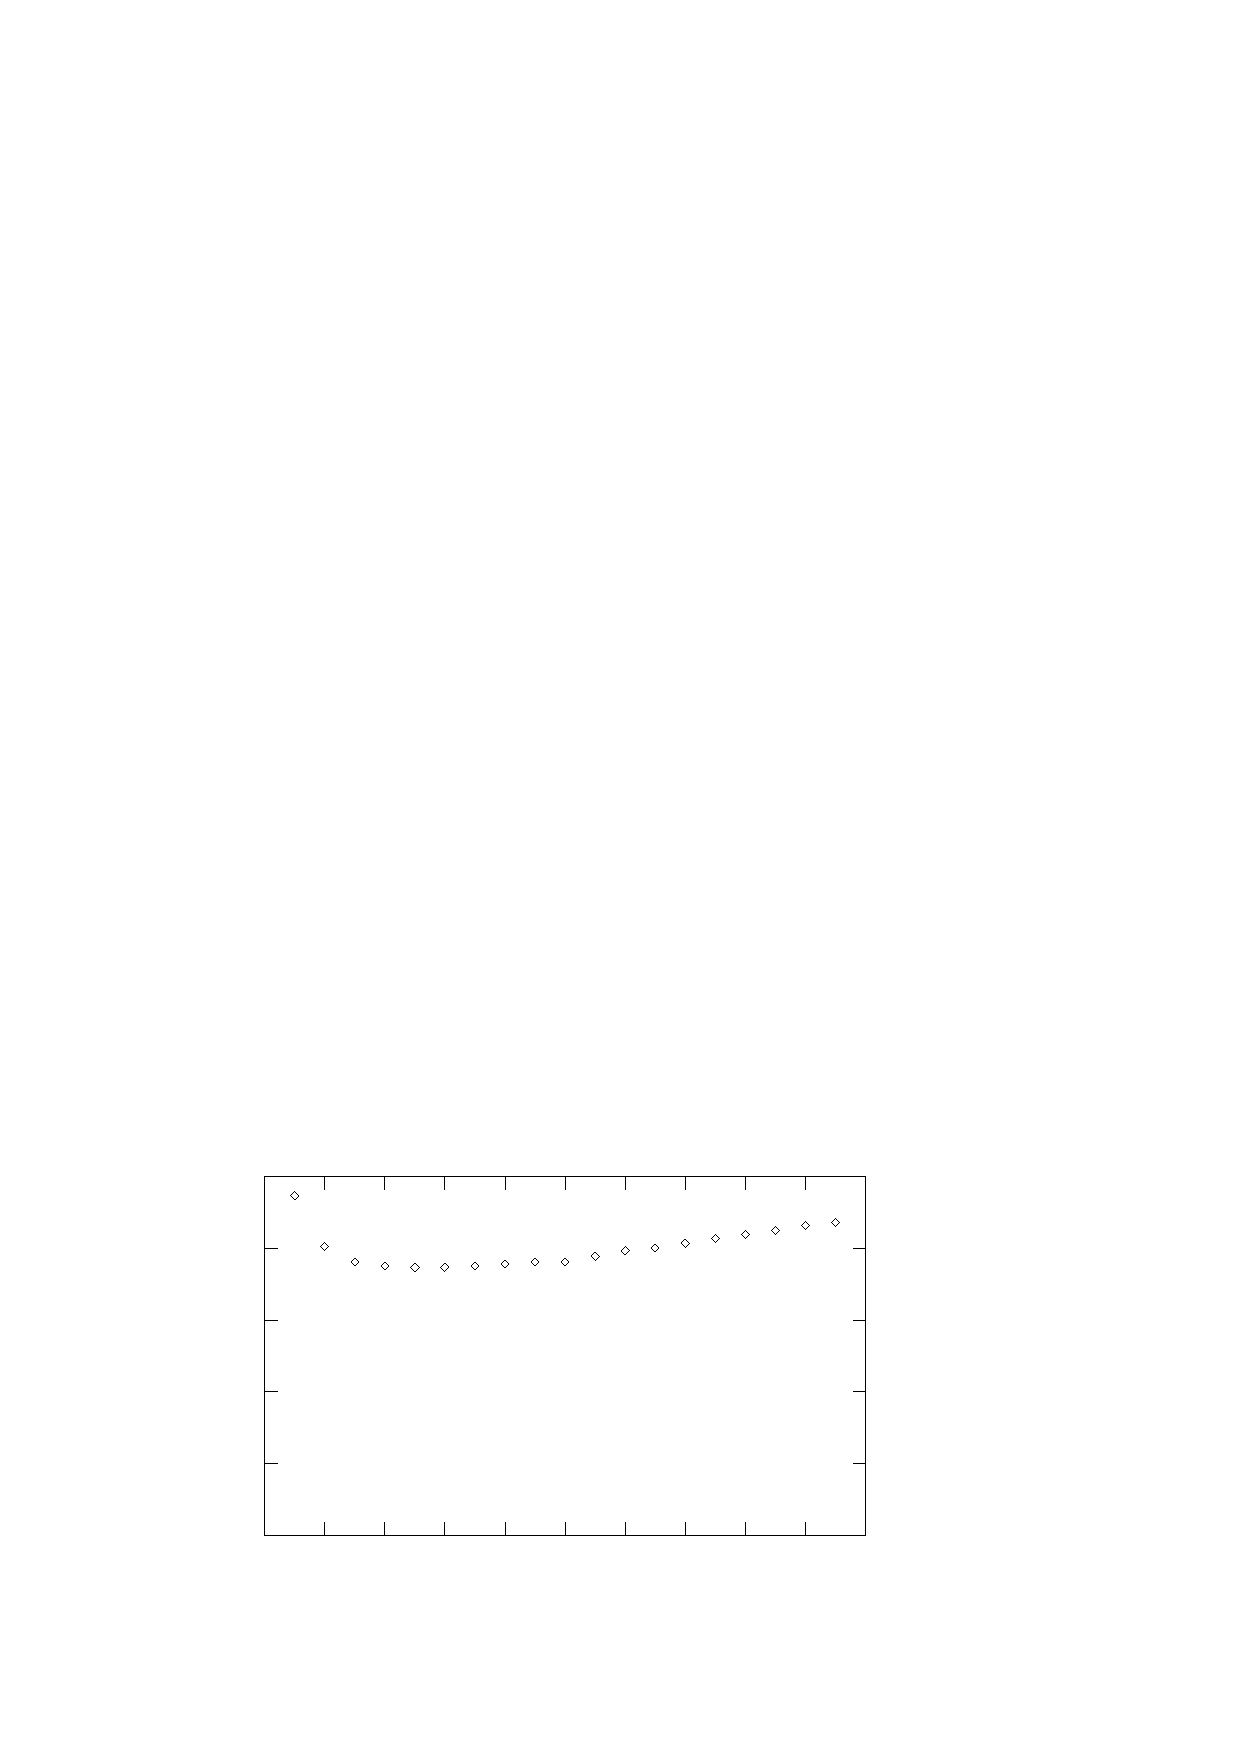
\includegraphics{diagram2}%
\end{picture}%
\setlength{\unitlength}{0.0200bp}%
\begin{picture}(18000,10800)(0,0)%
\put(2475,1650){\makebox(0,0)[r]{\strut{} 0}}%
\put(2475,3370){\makebox(0,0)[r]{\strut{} 0.05}}%
\put(2475,5090){\makebox(0,0)[r]{\strut{} 0.1}}%
\put(2475,6810){\makebox(0,0)[r]{\strut{} 0.15}}%
\put(2475,8530){\makebox(0,0)[r]{\strut{} 0.2}}%
\put(2475,10250){\makebox(0,0)[r]{\strut{} 0.25}}%
\put(2750,1100){\makebox(0,0){\strut{} 0}}%
\put(4193,1100){\makebox(0,0){\strut{} 2}}%
\put(5635,1100){\makebox(0,0){\strut{} 4}}%
\put(7078,1100){\makebox(0,0){\strut{} 6}}%
\put(8520,1100){\makebox(0,0){\strut{} 8}}%
\put(9963,1100){\makebox(0,0){\strut{} 10}}%
\put(11405,1100){\makebox(0,0){\strut{} 12}}%
\put(12848,1100){\makebox(0,0){\strut{} 14}}%
\put(14290,1100){\makebox(0,0){\strut{} 16}}%
\put(15733,1100){\makebox(0,0){\strut{} 18}}%
\put(17175,1100){\makebox(0,0){\strut{} 20}}%
\put(550,5950){\rotatebox{90}{\makebox(0,0){\strut{}ratio of page faults to accesses}}}%
\put(9962,275){\makebox(0,0){\strut{}shifting frequency in read-instructions per shift}}%
\end{picture}%
\endinput


\vspace{5mm}

Obviously, the best performance is achieved when shifting every 5
read-instructions.

\section{Summary}

These scripts help you to find the best page replacement algorithm for
a specific environment.

We did not simulate any real existing system environments, as this
would mean reinventing the wheel and there are too many of them.
These scripts are intended to be used at the designing phase of
\emph{new} hardware and operating systems.

\section{Bibliography}

\begin{thebibliography}{Tanenbaum, 2001 x}
\bibitem [Tanenbaum, 2001] {Tan01} Tanenbaum, A.\ S., Modern Operating
  Systems, Upper Saddle River 2001$^2$
\end{thebibliography}

\end{document}
